\tikzstyle{box} = [rectangle, rounded corners, minimum width=3.5cm, minimum height=1cm,text centered, draw=black]
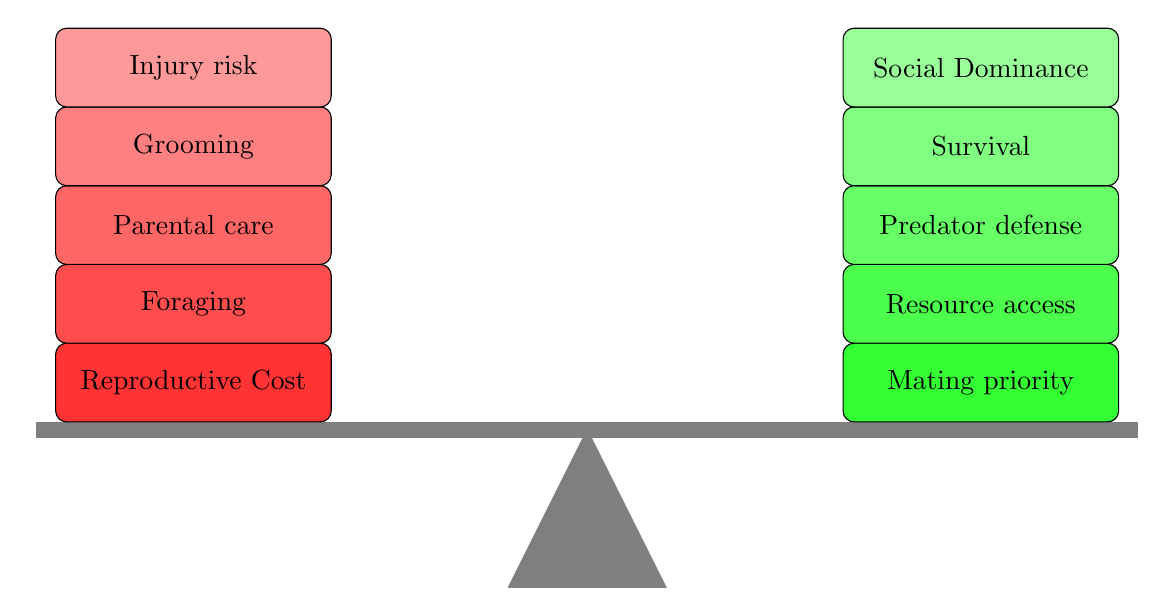
\begin{tikzpicture}
	\draw[line width=6, gray] (-7,0)-- (0,0) --(7,0);
	\draw[gray, fill=gray] (-1,-2)-- (0,0) --(1,-2) --(-1,-2);

	%Cost
	\node (injury) [box, fill=red!80] at (-5,0.6)  {Reproductive Cost};
	\node (grooming) [box, fill=red!70, above of=injury] {Foraging};
	\node (repo) [box, fill=red!60, above of=grooming] {Parental care};
	\node (foraging) [box, fill=red!50, above of=repo] {Grooming};
	\node (parCare) [box, fill=red!40, above of=foraging] {Injury risk};

	%Benefit
	\node (mat) [box, fill=green!80] at (5,0.6)  {Mating priority};
	\node (res) [box, fill=green!70, above of=mat] {Resource access};
	\node (def) [box, fill=green!60, above of=res] {Predator defense};
	\node (surv) [box, fill=green!50, above of=def] {Survival};
	\node (dom) [box, fill=green!40, above of=surv] {Social Dominance};

\end{tikzpicture}
